\documentclass{article}
\usepackage[utf8]{vietnam}
\usepackage{xcolor}

\usepackage{amsmath}
\usepackage{amssymb}

\usepackage{tabularx}
\usepackage{graphicx}
\usepackage{listings}
\usepackage{float}
\usepackage{setspace}

\bibliographystyle{ieeetr}

\definecolor{codegreen}{rgb}{0,0.6,0}
\definecolor{codegray}{rgb}{0.5,0.5,0.5}
\definecolor{codepurple}{rgb}{0.58,0,0.82}
\definecolor{backcolour}{rgb}{0.95,0.95,0.92}


\lstdefinestyle{mystyle}{
    backgroundcolor=\color{backcolour},   
    commentstyle=\color{codegreen},
    keywordstyle=\color{magenta},
    numberstyle=\tiny\color{codegray},
    stringstyle=\color{codepurple},
    basicstyle=\ttfamily\footnotesize,
    breakatwhitespace=false,         
    breaklines=true,                 
    captionpos=b,                    
    keepspaces=true,                 
    numbers=left,                    
    numbersep=5pt,                  
    showspaces=false,                
    showstringspaces=false,
    showtabs=false,                  
    tabsize=2
}

\lstset{style=mystyle}
\title{Pima2021}
\author{Long Nguyen}
\date{July 26, 2021}
\begin{document}
\maketitle
\tableofcontents
\pagebreak
\section{Mô tả bài toán}


\subsection{Bài toán 1}
Dữ liệu được đưa dưới dạng một danh sách các vector $D$ chiều được ký hiệu là: $X = (\vec{x}_1, \vec{x}_2, \ldots, \vec{x}_n)^T$ với $\vec{x}_i \in \mathbb{R}^d$. \\ 

Một phân phối chuẩn nhiều chiều định nghĩa bởi vector trung bình và $\vec{\mu}$ ma trận covariance $\Sigma$. Vector ngẫu nhiên $\vec{X}$  được gọi là tuân theo phân phối đều $D$ chiều ký hiệu là: $\vec{X} \sim N_D(\vec{\mu}, \Sigma)$, khi đó hàm mật độ xác suất có thể được tính như công thức \ref{congthuc1}
\begin{equation}
    f(\vec{x}; \vec{\mu}, \Sigma)
    = \dfrac{1}{\sqrt{(2\pi)^k|\Sigma|}} \exp{-\dfrac{1}{2} (\vec{x} - \vec{\mu}) \Sigma^{-1} (\vec{x}-\vec{\mu})^T}
    \label{congthuc1}
\end{equation}
\subsection{Bài toán 2}
Thầy Dũng muốn tham dự trại hè Pima 2022 ở Cape Town, Nam Phi. Tuy nhiên, do không có đường bay thẳng từ Thành phố Hồ Chí Minh đến Nam Phi nên thầy Dũng phải quá cảnh ở hai thành phố khác. Dựa vào bảng sau đây, hãy giúp thầy Dũng chọn lộ trình bay ít tốn kém nhất. Nguồn bài toán gốc từ bài giảng \cite{graph}.
\begin{table}[h]
    \centering
\begin{tabularx}{\linewidth}{|l|X|X|X|X|X|X|X|X|}\hline
 {}&HCM&Chia\-ngmai&Singa\-pore&Santa Marta&San Antonio&Los Angeles&Paris&Cape Town \\ \hline
  {{\text{HCM}}}& - &{250}&{176}&{1039}& - & - & - & -  \\ \hline
  {{\text{Chiangmai}}}& - & - & - & - &{1480}&{1565}&{647}& -  \\ \hline
  {{\text{Singapore}}}& - & - & - & - &{1733}& - &{546}& -  \\ \hline
  {{\text{Santa Marta}}}& - & - & - & - &{540}&{769}& - & -  \\ \hline
  {{\text{San Antonio}}}& - & - & - & - & - &{-}&{-}&{1103} \\ \hline
  {{\text{Los Angeles}}}& - & - & - & - & - & - &{-}&{967} \\ \hline
  {{\text{Paris}}}& - & - & - & - & - & - & - &{2016} \\\hline
  {{\text{Cape Town}}}& - & - & - & - & - & - & - & - \\ \hline
\end{tabularx}
\caption{Bảng trọng số đường bay giữa các trạm}
\end{table}

\subsection{Bài toán 3}
Sobel là một thuận toán phát hiện biên cạnh dựa theo gradient trên hướng x và y. Dưới đây là mô tả của thuật toán.

\begin{figure}[H]
    \centering
    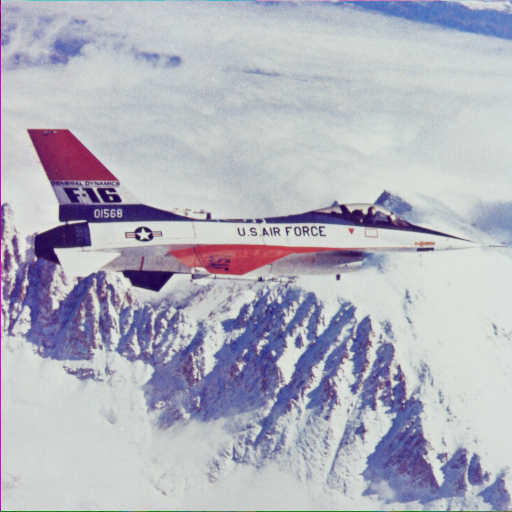
\includegraphics[width=0.45\textwidth]{airplane_raw.png}
    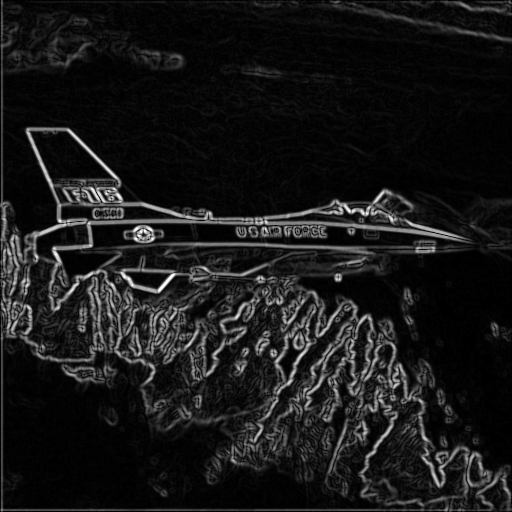
\includegraphics[width=0.45\textwidth]{airplane.png}
\end{figure}

Mã giả nguồn của thuật toán 
\begin{onehalfspace}
\begin{lstlisting}[language=Python]
def sobel_edge_detection(image, filter):
    import numpy as np
    im_x = convolution(image, filter)
    im_y = convolution(image, np.flip(filter.T, axis=0))
    gradient_magnitude = np.square(im_x) + np.square(im_y)
    gradient_magnitude = np.sqrt(gradient_magnitude)
    gradient_magnitude *= 255.0 / gradient_magnitude.max()
    return gradient_magnitude
\end{lstlisting}
\end{onehalfspace}
\bibliography{references}
\end{document}